\documentclass[english,serif,mathserif,xcolor=pdftex,dvipsnames,table]{beamer}
\usetheme[informal]{s3it}
\usepackage{s3it}

\title{%
  Python basics
}
\author[S3IT]{%
  S3IT: Services and Support for Science IT, \\
  University of Zurich
}
\date{Mar.~19--20, 2014}

\begin{document}

% title frame
\maketitle


\begin{frame}[fragile]
  \frametitle{The Python shell, I}
  Python is an \emph{interpreted} language.

  \+
  It also features an interactive
  \href{http://en.wikipedia.org/wiki/REPL}{``shell''} for evaluating
  expressions and statements immediately.

  \+
  The Python shell is started by invoking the command
  \texttt{python} in a terminal window.
\begin{semiverbatim}\small
\$ \textbf{python}
Python 2.7.1+ (r271:86832, Apr 11 2011, 18:13:53)
[GCC 4.5.2] on linux2
Type "help", "copyright", "credits" or "license"
for more information.
>>>
\end{semiverbatim}
\end{frame}

\begin{frame}[fragile]
  \frametitle{The Python shell, II}
  Expressions can be entered at the Python shell prompt (the
  `\texttt{>>>}' at the start of a line); they are evaluated and the
  result is printed:
\begin{semiverbatim}
>>> 2+2
4
\end{semiverbatim}

  \+
  A line can be continued onto the next by ending it with the
  character `\texttt{\textbackslash}'; for example:
\begin{semiverbatim}
>>> "hello" + \textbackslash
... " world!"
'hello world!'
\end{semiverbatim}
  The prompt changes to `\texttt{...}' on continuation lines.

  \+\scriptsize
  Reference:
  \url{http://docs.python.org/reference/lexical_analysis.html#line-structure}
\end{frame}


\begin{frame}
  \frametitle{Basic types}
  Basic object types in Python:
  \begin{description}
  \item[bool] The class of the two boolean constants \texttt{True}, \texttt{False}.
  \item[int] Integer numbers: \texttt{1}, \texttt{-2}, \ldots
  %   up to \texttt{9223372036854775807} (on a 64-bit machine)
  % \item[long] Integer numbers of arbitrary size; Python switches
  %   automatically from \texttt{int} to \texttt{long} when needed.
  \item[float] Double precision floating-point numbers, e.g.:
    \texttt{3.1415}, \texttt{-1e-3}.
  \item[str] Text (strings of byte-size characters).
  %\item[unicode] Strings of UNICODE characters.
  \item[list] Mutable list of Python objects
  \item[dict] Key/value mapping
  \end{description}

  \+
  The \texttt{list} and \texttt{dict} types are essential data
  structures, so we are covering them extensively afterwards.
\end{frame}

\begin{frame}[fragile]
  \frametitle{String literals, I}
  There are several ways to express string literals in Python.

  \+
  Single and double quotes can be used interchangeably:
\begin{semiverbatim}
>>> "a string" == 'a string'
True
\end{semiverbatim}

  \+
  You can use the single quotes inside double-quoted strings, and viceversa:
\begin{semiverbatim}
>>> a = "Isn't it ok?"
>>> b = '"Yes", he said.'
\end{semiverbatim}
\end{frame}


\begin{frame}[fragile]
  \frametitle{String literals, II}
  Multi-line strings are delimited by three quote characters.
\begin{lstlisting}[showstringspaces=false]
>>> a = """This is a string,
... that extends over more
... than one line.
... """
\end{lstlisting}

  \+ In other words, you need not use the backslashes
  ``\texttt{\textbackslash}'' at the end of the lines.
\end{frame}


\begin{frame}[fragile]
  \frametitle{Operators}
  All the usual unary and binary arithmetic operators are
  defined in Python: \texttt{+}, \texttt{-}, \texttt{*}, \texttt{/},
  \texttt{**}~(exponentiation), \texttt{<<}, \texttt{>>}, etc.

  \+
  Logical operators are expressed using plain English words:
  \texttt{and}, \texttt{or}, \texttt{not}.

  \+
  Numerical and string comparison also follows the usual notation:
  \texttt{<}, \texttt{>}, \texttt{<=}, \texttt{==}, \texttt{!=},
  \ldots

  \+
  \begin{references}
    \tiny
    \begin{itemize}
    \item
      \url{http://docs.python.org/library/stdtypes.html#boolean-operations-and-or-not}
    \item
      \url{http://docs.python.org/library/stdtypes.html#comparisons}
    \end{itemize}
  \end{references}
\end{frame}


\begin{frame}
  \frametitle{Your first exercise}
  %\href{http://www.pythonchallenge.com}{\includegraphics[width=\linewidth]{fig/2to38}}
  \begin{center}
    {\Large How much is \href{http://www.pythonchallenge.com}{$2^{38}$} ?}

    \+
    (You have 2 minutes' time.)
  \end{center}
\end{frame}


\begin{frame}[fragile]
  \frametitle{Operators, II}
  Some operators are defined for non-numeric types:
\begin{lstlisting}
>>> "U" + 'ZH'
'UZH'
\end{lstlisting}

  \+
  Some support operands of mixed type:
\begin{lstlisting}
>>> "a" * 2
'aa'
>>> 2 * "a"
'aa'
\end{lstlisting}

  \+
  Some do not:
\begin{lstlisting}[basicstyle=\footnotesize\ttfamily]
>>> "aaa" / 3
Traceback (most recent call last):
  File "<stdin>", line 1, in <module>
TypeError: unsupported operand type(s) for /: 'str' and 'int'
\end{lstlisting}
\end{frame}


\begin{frame}[fragile]
  \frametitle{Operators, III}
  The ``\texttt{\%}'' operator computes the remainder of integer division.
  \begin{lstlisting}
    >>> 9 % 2
    1
  \end{lstlisting}
\end{frame}


\begin{frame}[fragile]
  \frametitle{Operators, IV}
  The ``\texttt{\%}'' operator is also used for \emph{string
    formatting}:
\begin{lstlisting}
>>> "This is slide ~\alt<2>{\HL{\%d}}{\%d}~ of %d" % (~\alt<2>{\HL{11}}{11}~, 32)
'This is slide 11 of 32.'
>>> "We are ~\alt<3>{\HL{\%.1f}}{\%.1f}~%% done." % (~\alt<3>{\HL{100.0 * 11/32}}{100.0 * 11/32}~)
'We are 40.6% done.'
>>> "Today is ~\alt<4>{\HL{\%s}}{\%s}~ %d, %d" % (~\alt<4>{\HL{'September'}}{'September'}~, 11, 2012)
'Today is October 28, 2012'
\end{lstlisting}

  \only<2>{The \texttt{\%d} in the left string is substituted with the
    base-10 representation of the integer number on the right side.}
  \only<3>{The \texttt{\%f} in the left string is substituted with the
    floating-point number on the right side; the number of digits to
    put after the comma is written \emph{before} the \texttt{f}}
  \only<4>{The \texttt{\%s} in the left string is substituted with the
    string on the right side.}

  \begin{references}
    \url{http://docs.python.org/library/stdtypes.html#string-formatting-operations}
  \end{references}
\end{frame}


% \begin{frame}[fragile]
%   \frametitle{Expressions}

%   Expressions are combinations of operations that manipulate values
%   and return some other values.  (Function calls are operations, too.)

%   \+
%   For instance, \texttt{2+2} is an expression, as are
%   \texttt{abs(-2)}, \texttt{os.path.exists('/tmp')},
%   \texttt{1 + (1.0/2) + 2**(-2)}

%   \+
%   \emph{Not all Python constructs return a value.}
%   (Assignment, for example, does not.)

%   \+\scriptsize
%   References:
%   \url{http://lambda-the-ultimate.org/node/1044#comment-10878}
%   \url{http://docs.python.org/reference/expressions.html}

% \end{frame}


\begin{frame}[fragile]
  \frametitle{Assignment, I}
  Assignment is done via the `\texttt{=}' statement:
\begin{semiverbatim}
>>> a = 1
>>> print(a)
1
\end{semiverbatim}

  \+
  There are a few shortcut notations:
  \begin{itemize}
  \item[] \texttt{\emph{a} += \emph{b}} short for \texttt{\emph{a} = \emph{a} + \emph{b}},
  \item[] \texttt{\emph{a} -= \emph{b}} short for \texttt{\emph{a} = \emph{a} - \emph{b}},
  \item[] \texttt{\emph{a} *= \emph{b}} short for \texttt{\emph{a} = \emph{a} * \emph{b}},
  \item[]   etc. --- one for every legal operator.
  \end{itemize}
\end{frame}


\begin{frame}[fragile]
  \frametitle{Assignment, II}

  \textbf{Python variables are just ``names'' given to values.}
  This allows you to \emph{reference} the string \texttt{'Python'}
  by the \emph{name} \texttt{a}:

  \+
  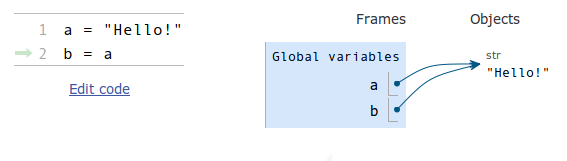
\includegraphics[width=1\linewidth]{fig/a=b.png}

  \+
  The same object can be given many names!

  \+
  \begin{seealso}
    \scriptsize \url{http://excess.org/article/2014/04/bar-foo/}
  \end{seealso}
\end{frame}


\begin{frame}[fragile]
  \frametitle{The \texttt{is} operator}

  The \texttt{is} operator allows you to test whether two names refer
  to the same object:
\begin{lstlisting}
>>> a = 1
>>> b = 1
>>> a is b
True
\end{lstlisting}

\end{frame}


\begin{frame}[fragile,label=func1]
  \frametitle{Functions, I}
  Functions are called by postfixing the function name with a
  parenthesized argument list.

  \+
\begin{lstlisting}
>>> int("42")
42
>>> int(4.2)
4
>>> float(42)
42.0
>>> str(42)
'42'
>>> str()
''
\end{lstlisting}

  \hyperlink{typeconv}{\beamergotobutton{More on int, float, str}}
\end{frame}


\begin{frame}[fragile]
  \frametitle{Functions, II}
  Some functions can take a variable number of arguments:
  \begin{description}
    % \item[sum($x_0$, \ldots, $x_n$)] Return $x_0 + \cdots + x_n$.
    \item[max($x_0$, \ldots, $x_n$)] Return the maximum of the set $\{ x_0, \ldots, x_n \}$
    \item[min($x_0$, \ldots, $x_n$)] Return the minimum of the set $\{ x_0, \ldots, x_n \}$
  \end{description}

  \+
  Examples:
\begin{semiverbatim}
>>> min(1,2,3)
1
>>> max(1,2)
2
\end{semiverbatim}
\end{frame}


\begin{frame}[fragile]
  \frametitle{The most important function of all}
  \begin{description}
  \item[help(\texttt{fn})] Display help on the function named \texttt{fn}
  \end{description}

  \+
  \begin{question}
    What happens if you type these at the prompt?
    \begin{itemize}
    \item \texttt{help(abs)}
    \item \texttt{help(max)}
    \end{itemize}
  \end{question}
\end{frame}

% \begin{frame}
%   \frametitle{The most important function of all, II}

%   When called without any argument, \hl{help()} starts an interactive
%   help prompt.

%   \+
%   \begin{semiverbatim}\tiny
% >>> help()

% Welcome to Python 2.7!  This is the online help utility.

% If this is your first time using Python, you should definitely check out
% the tutorial on the Internet at http://docs.python.org/tutorial/.

% Enter the name of any module, keyword, or topic to get help on writing
% Python programs and using Python modules.  To quit this help utility and
% return to the interpreter, just type "quit".

% To get a list of available modules, keywords, or topics, type "modules",
% "keywords", or "topics".  Each module also comes with a one-line summary
% of what it does; to list the modules whose summaries contain a given word
% such as "spam", type "modules spam".

% help>
% \end{semiverbatim}

%   \+
%   To return to the normal prompt, type \texttt{quit}

%   \+
%   \hl{help(\texttt{'topic'})} has the same effect as typing
%   \texttt{topic} at the interactive help prompt.
% \end{frame}

\begin{frame}[fragile]
  \frametitle{How to define new functions}
  \begin{columns}[t]
    \begin{column}{0.5\textwidth}
\begin{lstlisting}
~\HL{\textbf{def} greet(name):}~
  """
  A friendly function.
  """
  print ("Hello, " + name + "!")

# the customary greeting
greet("world")
\end{lstlisting}
    \end{column}
    \begin{column}{0.5\textwidth}
      \raggedleft
      The \textbf{def} statement starts a function definition.
    \end{column}
  \end{columns}
\end{frame}

\begin{frame}[fragile]
  \begin{columns}[t]
    \begin{column}{0.5\textwidth}
\begin{lstlisting}
def greet(name):
  """
  A friendly function.
  """
  ~\HL{print ("Hello, " + name + "!")}~

# the customary greeting
greet("world")
\end{lstlisting}
    \end{column}
    \begin{column}{0.5\textwidth}
      \raggedleft
      \textbf{Indentation is significant in Python}: it is used to delimit
      blocks of code, like `\texttt{\{}' and `\texttt{\}}' in Java and C.
    \end{column}
  \end{columns}
\end{frame}

\begin{frame}[fragile]
  \begin{columns}[t]
    \begin{column}{0.5\textwidth}
\begin{lstlisting}
def greet(name):
  """
  A friendly function.
  """
  print ("Hello, " + name + "!")

~\HL{\it\tt\#\ the customary greeting}~
greet("world")
\end{lstlisting}
    \end{column}
    \begin{column}{0.5\textwidth}
      \raggedleft
      (This is a comment. It is ignored by Python, just like blank lines.)
    \end{column}
  \end{columns}
\end{frame}

\begin{frame}[fragile]
  \begin{columns}[t]
    \begin{column}{0.5\textwidth}
\begin{lstlisting}
def greet(name):
  """
  A friendly function.
  """
  print ("Hello, " + name + "!")

# the customary greeting
~\HL{greet("world")}~
\end{lstlisting}
    \end{column}
    \begin{column}{0.5\textwidth}
      \raggedleft
      This calls the function just defined.
    \end{column}
  \end{columns}
\end{frame}

\begin{frame}[fragile]
  \begin{columns}[t]
    \begin{column}{0.5\textwidth}
\begin{lstlisting}
def greet(name):
  ~\HL{"""}~
  ~\HL{A friendly function.}~
  ~\HL{"""}~
  print ("Hello, " + name + "!")

# the customary greeting
greet("world")
\end{lstlisting}
    \end{column}
    \begin{column}{0.5\textwidth}
      \raggedleft
      What is this? The answer in the next exercise!
    \end{column}
  \end{columns}
\end{frame}

\begin{frame}
  \begin{exercise}
    Type and run the code on the previous page at the interactive
    prompt. (Type indentation spaces, too!)

    What does \texttt{help(greet)} print?
    What's the result of evaluating the function \texttt{greet("world")}?
  \end{exercise}

  \+
  \begin{exercise}
    Type the same code in a file named \texttt{hello.py}, then type
    \texttt{import hello} at the interactive prompt.
    What happens?  Type \texttt{import hello} again; what happens?
  \end{exercise}

  \+
  \begin{exercise}
    At the terminal, type \texttt{python hello.py}.  What happens?
    Type it again; what happens?
  \end{exercise}
\end{frame}


\begin{frame}[fragile]
  \frametitle{Modules, I}
  The \texttt{import} statement reads a \texttt{.py} file, executes
  it, and makes its contents available to the current program.
\begin{lstlisting}
>>> import hello
Hello, world!
\end{lstlisting}

  \+
  \textbf{Modules are only read once}, no matter how many times an
  \texttt{import} statement is issued.
\begin{lstlisting}
>>> import hello
Hello, world!
>>> import hello
>>> import hello
\end{lstlisting}

\end{frame}


\begin{frame}[fragile]
  \frametitle{Modules, II}
  Modules are \emph{namespaces:} functions and variables defined in
  a module must be prefixed with the module name when used in other
  modules:
\begin{lstlisting}
>>> hello.greet("Bob")
Hello, Bob!
\end{lstlisting}

  \+
  To import definitions into the current namespace, use the
  `\texttt{from $x$ import $y$}' form:
\begin{lstlisting}
>>> from hello import greet
>>> greet("Bob")
Hello, Bob!
\end{lstlisting}
\end{frame}


\begin{frame}[fragile]
  \frametitle{The `return` statement}

  \begin{columns}
    \begin{column}{0.5\textwidth}
      \begin{lstlisting}
def double(x):
  ~\HL{return x+x}~

double(3) == 6
      \end{lstlisting}
    \end{column}
    \begin{column}{0.5\textwidth}
      \raggedleft The result of a function evaluation is set by the
      \textit{return} statement.

     \+
      If no \texttt{return} is present, the function returns the
      special value \texttt{None}.

         \end{column}
  \end{columns}
\+
  \begin{columns}
    \begin{column}{0.5\textwidth}
      \begin{lstlisting}
def double(x):
  return x+x
  # the following line
  # is never exec'd
  ~\HL{print('Hello')}~
      \end{lstlisting}
    \end{column}
    \begin{column}{0.5\textwidth}
      \raggedleft After executing \texttt{return} the control flow
      leaves the function.
    \end{column}
  \end{columns}

\end{frame}

%%% Conditionals

\begin{frame}[fragile]
  \frametitle{Conditionals}
  Conditional execution uses the \texttt{if} statement:
\begin{lstlisting}
if ~\it expr~:
  # indented block
elif ~\it other-expr~:
  # indented block
else:
  # executed if none of the above matched
\end{lstlisting}

  \+The \texttt{elif} can be repeated, with different conditions, or
  left out entirely.

  \+
  Also the \texttt{else} clause is optional.

  \+
  \begin{question}
    Where's the `end if'?

    \pause{There's no `end if': indentation delimits blocks!}
  \end{question}
\end{frame}


\begin{frame}[fragile]
  \frametitle{Looping}
  Conditional looping uses the \texttt{while} statement:
\begin{lstlisting}
while ~\it expr~:
  # indented block
\end{lstlisting}
% else:
%   # executed at natural end of the loop

  \+
  To break out of a \texttt{while} loop, use the \texttt{break}
  statement.

  \+
  Use the \texttt{continue} statement anywhere in the indented
  block to jump back to the \texttt{while} statement.

  % \+
  % If a loop is exited via a \texttt{break} statement, the
  % \texttt{else} clause is \emph{not} executed.

  % \+
  % The \texttt{else} clause is optional.
\end{frame}


\begin{frame}
  \begin{exercise}
    In the \texttt{hello.py} file, modify the \texttt{greet()}
    function to print ``Welcome back!'' if the argument \texttt{name}
    is your name.

    \+
    Insert at least two distinct invocations of the function with
    different names at the end of the file.  Check that everything
    works by running \texttt{python hello.py} at the terminal prompt.
    (Or \emph{Ctrl+Shift+F10} in PyCharm.)
  \end{exercise}
\end{frame}


\begin{frame}[fragile,label=typeconv]
  \frametitle{Type conversions}
  \begin{description}
  \item[str($x$)] Converts the argument $x$ to a string; for numbers,
    the base 10 representation is used.
  \item[int($x$)] Converts its argument $x$ (a number or a string) to an integer;
    if $x$ is a a floating-point literal, decimal digits are truncated.
  \item[float($x$)] Converts its argument $x$ (a number or a string) to a
    floating-point number.
  \end{description}

  \hyperlink{func1}{\beamergotobutton{Back to Functions, I}}
\end{frame}


\begin{frame}
  \frametitle{Recap}
  \begin{enumerate}
  \item Indentation is used to delimit blocks of code!
  \item Variables are just names, a reference to real object.
  \item \lstinline|def function(arg1, arg2, ...):| to define functions
  \item \lstinline|import filename| to use code from other files.
  % \item Modules are \textit{namespaces}.
  % \item Conversion between types with \lstinline|int(), float(), str()| functions.
  \item To get information on something: \lstinline|help(something)|
  \end{enumerate}
\end{frame}


\end{document}


%%% Local Variables:
%%% mode: latex
%%% TeX-master: t
%%% End:
